\documentclass[a4paper,12pt]{article}
\usepackage{tikz}
\usepackage{amsmath,amssymb,amsthm,enumitem, amsfonts,listings,upquote, graphicx, color}
\usepackage[document]{ragged2e} %left justifies everything automatically
\usepackage{algorithm, algpseudocode}
\usepackage{fancyref}
\usepackage{color} %red, green, blue, yellow, cyan, magenta, black, white
\usepackage{apacite}
\usepackage{geometry}
\usepackage{adjustbox}
\usepackage{listings}  
\usepackage{graphicx}
\usepackage{float}
\usepackage{tabularx}


\DeclareMathOperator{\prox}{\mathbf{prox}}
\DeclareMathOperator*{\argmin}{arg\,min}

\newcommand{\N}{\mathbb{N}}
\newcommand{\Z}{\mathbb{Z}}

\newcommand\norm[1]{\left\lVert#1\right\rVert}

\lstset{ 
  tabsize=1,
  showstringspaces=false,
  breaklines=true,
}

\addtolength{\oddsidemargin}{-.875in}
\addtolength{\evensidemargin}{-.875in}
\addtolength{\textwidth}{1.75in}
\addtolength{\topmargin}{-.875in}
\addtolength{\textheight}{1.75in}

\definecolor{mygreen}{RGB}{28,172,0} % color values Red, Green, Blue
\definecolor{mylilas}{RGB}{170,55,241}
%%% FIX BELOW
\usepackage{blindtext}
\title{ECS 174 Project 1}
\author{
  Jiayi Lei\\
  SID: 915016668\\
  Email: cjlei@ucdavis.edu
  \and
  Zhengfeng Lai\\
  SID :916678034 \\
  Email: lzhengfeng@ucdavis.edu
} 

%%%\date{SQ 2019}
\date{\today}

\begin{document}
\maketitle
\begin{section}{I. Short Answer Problems}
\begin{subsection}{1}
For example if f and g are 3 by 3 filter, h is the original matrix with size of 100 by 100. By associative property of convolution, 


If we apply filter g and then filter f to image h respectively, we will have 100 * 100 * 3 * 3  + 100 * 100 * 3 * 3  = 180000 multiplications. However, if we apply the associative property of convolution, 
$$ f * (g * h) = (f * g) * h $$
we combine the two filters first and then apply the combined filter to the image. By doing this, we have 3* 3 * 3 = 27 multiplications to create the 3 by 3 combined filter and then it takes 100 * 100 * 3 * 3 = 90000 multiplicatoins to filter the image. totally 90027 multiplications, which is much more efficient than the previouse method. 

\end{subsection}

\begin{subsection}{2}
[1,1,1,1,1,0,1,1]

\end{subsection}

\begin{subsection}{3}
Addictive Gaussian noise might not presere image brightnees since the intensity of all pixels will go up. What's more, Gaussian noise is for random noise in the given image, there is chance that the recent noise created position might concide with earlier noise locations.

\end{subsection}

\begin{subsection}{4}
Assumption:\\
The time for producing one unit of product is the same for all assemblies, regardeless of whether there is flaw in the assembly. 

Method:\\
Step 1: Prerecord an assembly process which we are sure that there is no flaw on. Denote the time between two products passing the camera as t. Take out 10 key images with equal amount of time distance and denote those ten pictures as the standard pictures $s_1,s_2, s_3,..,s_10$\\
Step 2: During each t time laps, take out 10 key images for every t / 10 time laps. Lable those 10 key images as $t_1,t_2,t_3,...,t_10$\\

Step 3: Compare image $t_i$ to $s_i$, for all $i = 1, 2,3,...,10$.\\
step 3.1: Cluster based on intensity similarity to seperate the product from the backgroud of the belt, in order to reduced the difference or noice from the conveyor belt. \\
step 3.2:Smooth the picutures to suppress noice by using Gaussian filter. Enhace the edges by using contrast filter and localize the edges.
step 3.3: Compare the pitures with edges by using subtraction.\\


\end{subsection}

\end{section}


\begin{section}{II. Short Answer Problems}
\begin{subsection}{II.1}
Matlab CODE (seam\_carving\_decrease\_width.m):\\
\begin{lstlisting}[frame=single]  % Start your code-block
%seam_carving_decrease_width.m 
%Reduces the width of the image by 100 pixels

%%  inputSeamCarvingPrague.jpg
clc;clf;clear all;
im = imread('inputSeamCarvingPrague.jpg');
%imshow(reducedColorImg);
energyImg = energy_img(im);
for i = 1:100
    [im,~] = decrease_width(im,energyImg);
    energyImg = energy_img(im);
end
imshow(im);
imwrite(im,'outputReduceWidthPrague.png');

%%  inputSeamCarvingMall.jpg
clc;clf;clear all;
im = imread('inputSeamCarvingMall.jpg');
%imshow(reducedColorImg);
energyImg = energy_img(im);
for i = 1:100
    [im,~] = decrease_width(im,energyImg);
    energyImg = energy_img(im);
end
imshow(im);
imwrite(im,'outputReduceWidthMall.png');

\end{lstlisting}

OUTPUT:\\
\begin{figure}[!htb]
        \center{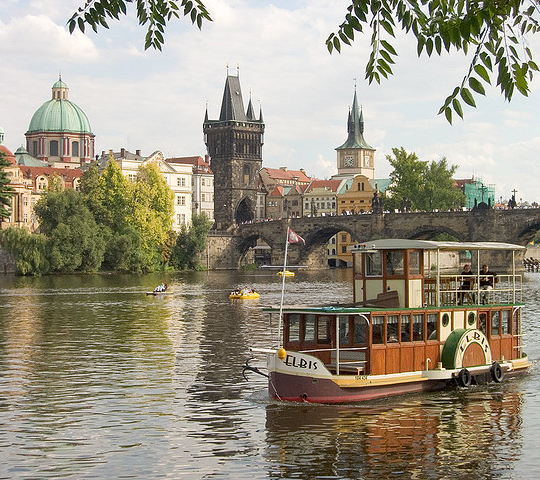
\includegraphics[width=\textwidth]
        {outputReduceWidthPrague.png}}
        \caption{outputReduceWidthPrague.png}
      \end{figure}
      
      
\begin{figure}[!htb]
        \center{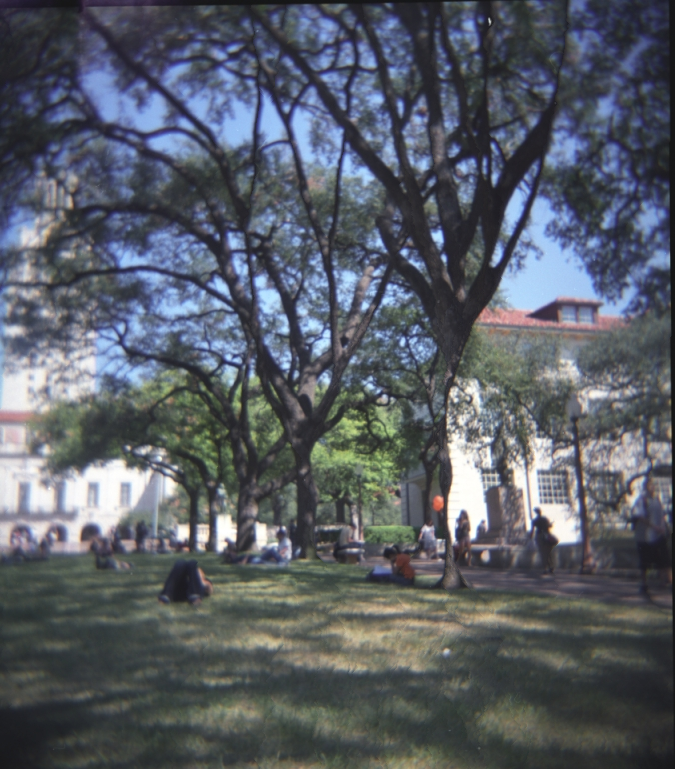
\includegraphics[width=\textwidth]
        {outputReduceWidthMall.png}}
        \caption{outputReduceWidthMall.png}
\end{figure}

\end{subsection}
\clearpage

\begin{subsection}{II.2}
Matlab CODE(seam\_carving\_decrease\_height.m):\\
\begin{lstlisting}[frame=single]  % Start your code-block
%seam_carving_decrease_height.m
%Reduce the height by 50 pixels

%%  inputSeamCarvingPrague.jpg
clc;clf;clear all;
reducedColorImg = imread('inputSeamCarvingPrague.jpg');
%imshow(reducedColorImg);
energyImg = energy_img(reducedColorImg);
for i = 1:50
    [reducedColorImg,~] = decrease_height(reducedColorImg,energyImg);
    energyImg = energy_img(reducedColorImg);
end
imshow(reducedColorImg);
imwrite(reducedColorImg,'outputReduceHeightPrague.png');

%%  inputSeamCarvingMall.jpg
clc;clf;clear all;
reducedColorImg = imread('inputSeamCarvingMall.jpg');
%imshow(reducedColorImg);
energyImg = energy_img(reducedColorImg);
for i = 1:50
    [reducedColorImg,~] = decrease_height(reducedColorImg,energyImg);
    energyImg = energy_img(reducedColorImg);
end
imshow(reducedColorImg);
imwrite(reducedColorImg,'outputReduceHeightMall.png');

\end{lstlisting}

OUTPUT:\\

\begin{figure}[!htb]
        \center{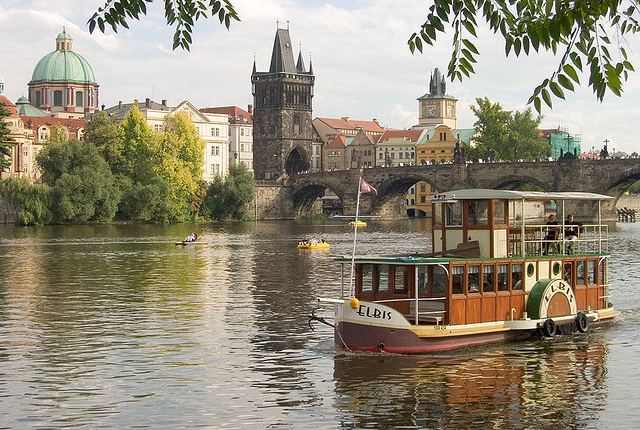
\includegraphics[width=\textwidth]
        {outputReduceHeightPrague.png}}
        \caption{outputReduceHeightPrague.png}
      \end{figure}




\begin{figure}[!htb]
        \center{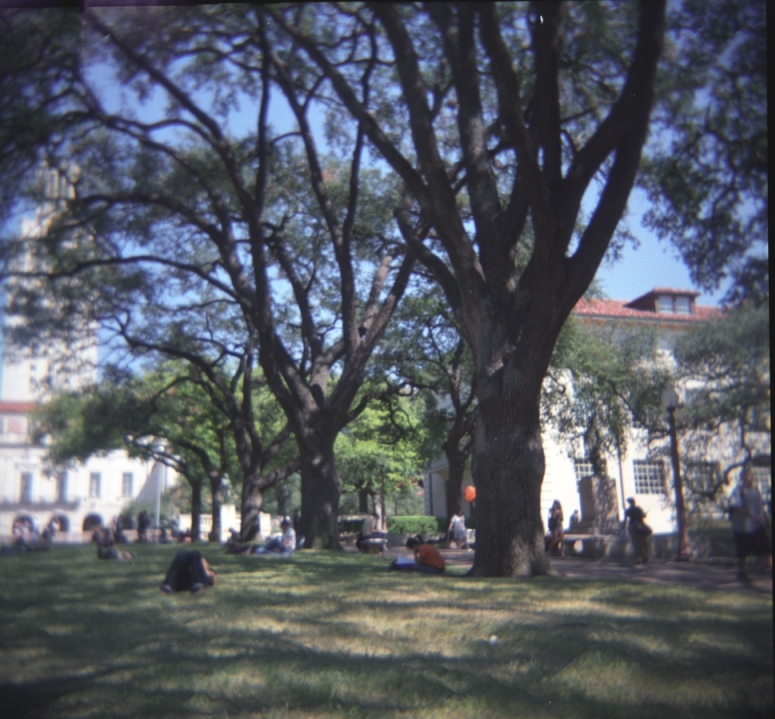
\includegraphics[width=\textwidth]
        {outputReduceHeightMall.png}}
        \caption{outputReduceHeightMall.png}
      \end{figure}
\end{subsection}

\clearpage

\begin{subsection}{II.3}



\begin{subsubsection}{a}
\begin{figure}[!htb]
        \center{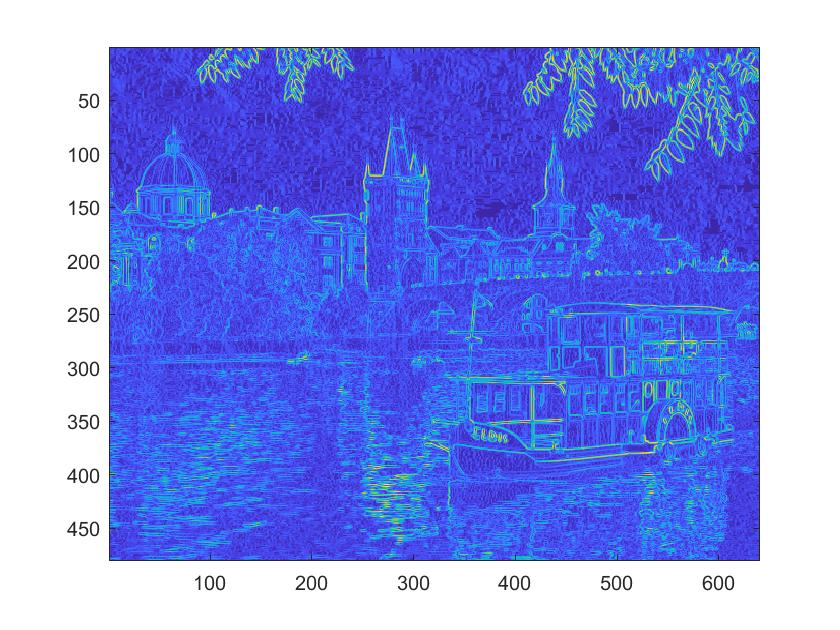
\includegraphics[width=\textwidth]
        {Problem3_a.jpg}}
        \caption{the energy function output for the provided image}
      \end{figure}
\end{subsubsection}

\clearpage
\begin{subsubsection}{b}

\begin{figure}[!htb]
        \center{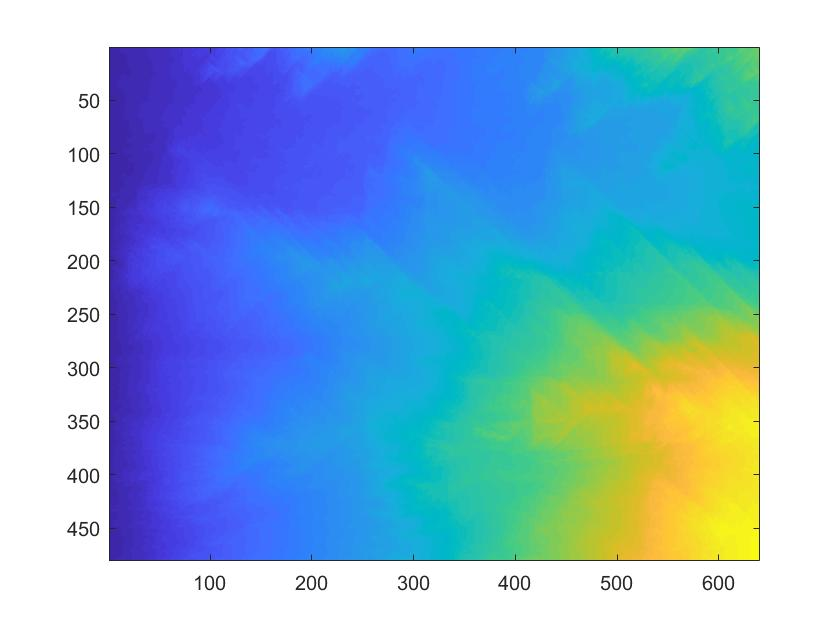
\includegraphics[width=\textwidth]
        {Problem3_b_horizontal.jpg}}
        \caption{cumulative minimum energy maps fro the seams in horizontal direction}
      \end{figure}
      
      \begin{figure}[!htb]
        \center{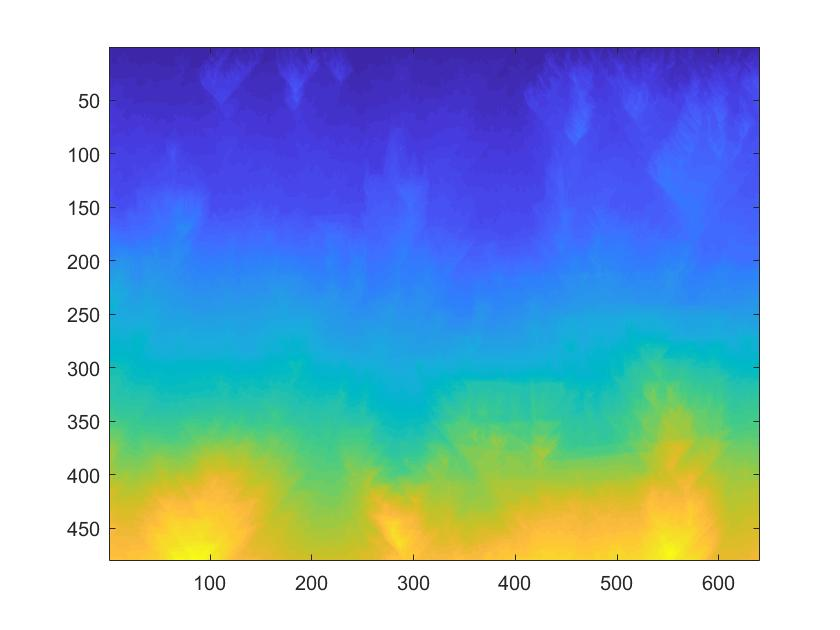
\includegraphics[width=\textwidth]
        {Problem3_b_vertical.jpg}}
        \caption{cumulative minimum energy maps fro the seams in vertical direction}
      \end{figure}
 \end{subsubsection}  
      \textbf {Explain why these outputs look the way they do given the original image’s content.}
The energy function output includes the outlines of the edges in the original image, successfully delineating key components when we calculate the minimum cost path. The cumulative minimum energy draws the key components with more clear details. The light areas corresponding to high energy cost at the bottom of the vertical energy map and on the right of the horizontal energy map. This is because the cumulative energy map function sweeps from top to bottom for vertical while left to right for horizontal. In the horizontal cumulative energy map, we can see high energy is at the large boat, buildings and bridges because we cannot start compressing the boat when we carve the original image horizontally. The vertical cumulative energy map places high energy cost at the boat and highly reflective areas of the water. The boats are the key component which cannot be carved.



\end{subsection}

\clearpage
\begin{subsection}{II.4}


\begin{figure}[!htb]
        \center{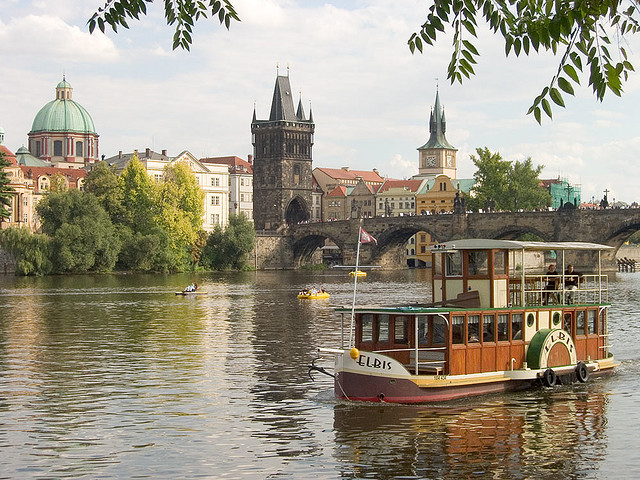
\includegraphics[width=\textwidth]
        {inputSeamCarvingPrague.jpg}}
        \caption{Original image}
      \end{figure}
            \clearpage
      
      
\begin{subsubsection}{(a)}
\begin{figure}[!htb]
        \center{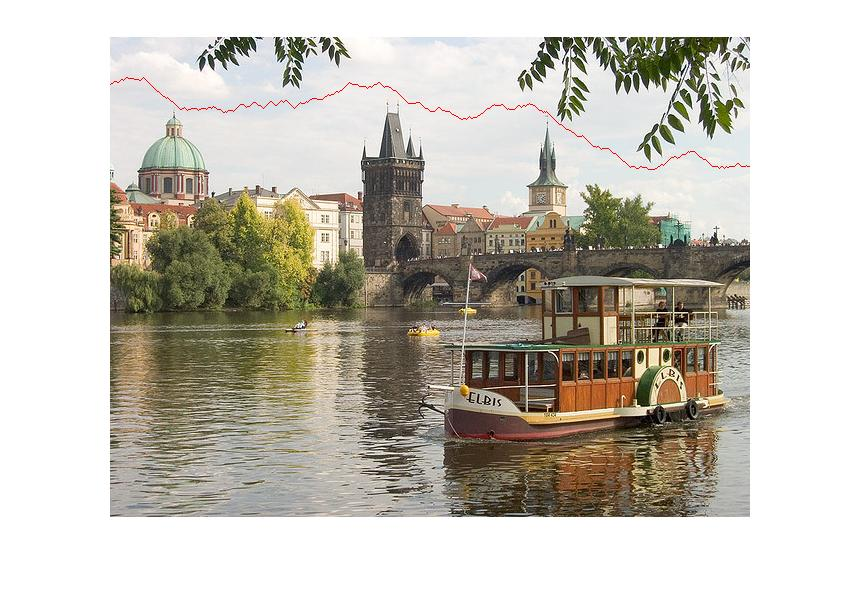
\includegraphics[width=\textwidth]
        {Problem4_Horizontal.jpg}}
        \caption{First selected horizontal seam}
      \end{figure}
      \clearpage
\end{subsubsection}
      \begin{subsubsection}{(b)}
      \begin{figure}[!htb]
        \center{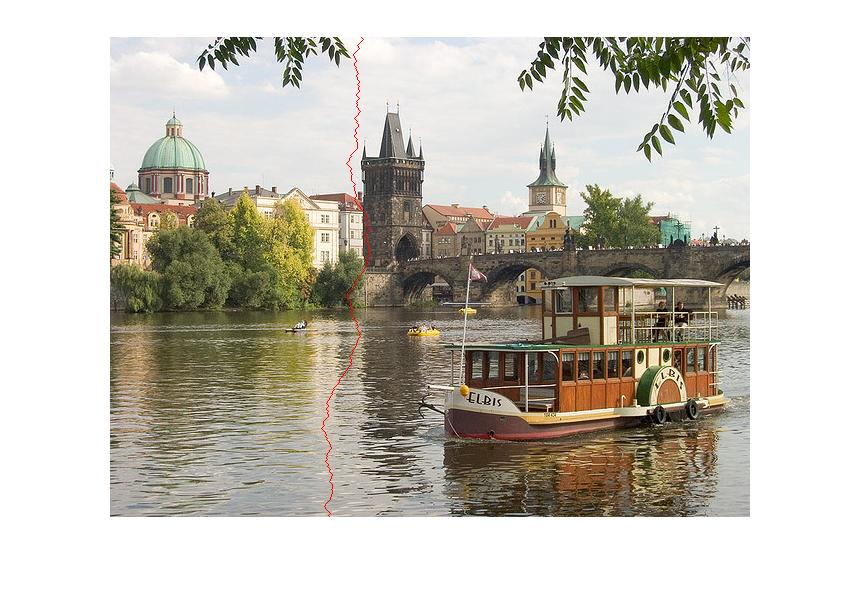
\includegraphics[width=\textwidth]
        {Problem4_Vertical.jpg}}
        \caption{First selected vertical seam}
      \end{figure}
	\end{subsubsection}
	      \clearpage
\textbf{Explain why these are the optimal seams for this image.}
The first vertical seam, nearly a vertical line, is around the edge of between the dark tower and the white building. The vertical seam also goes along the reflection of the white building in the water because the colors there are almost the same, which indicates low cost there. 
The first horizontal seam is in the sky where color is almost the same and the contrast is low. So there is low cost to seam at that place.


\end{subsection}

\clearpage
\begin{subsection}{II.5}


\begin{figure}[!htb]
        \center{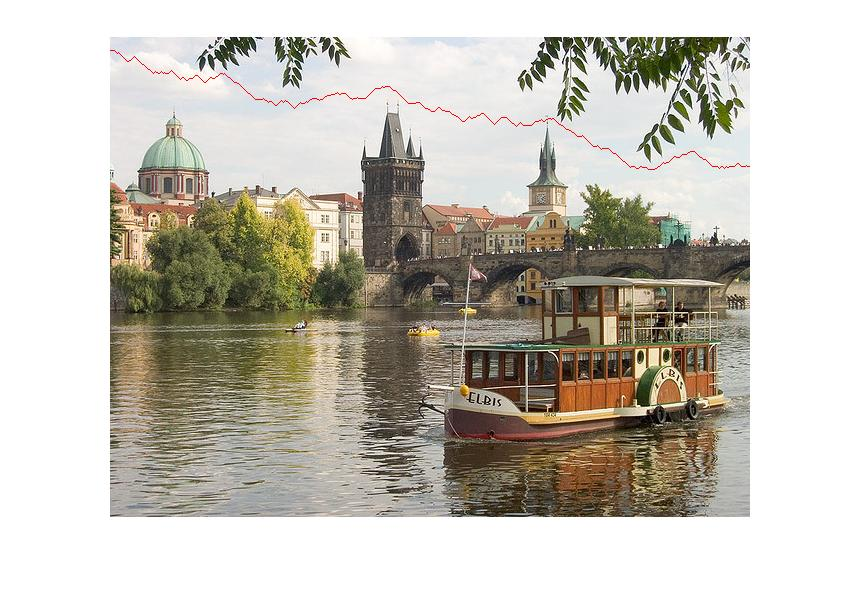
\includegraphics[width=\textwidth]
        {Problem5_horizontal.jpg}}
        \caption{First horizontal seam}
      \end{figure}
      \clearpage
      
      \begin{figure}[!htb]
        \center{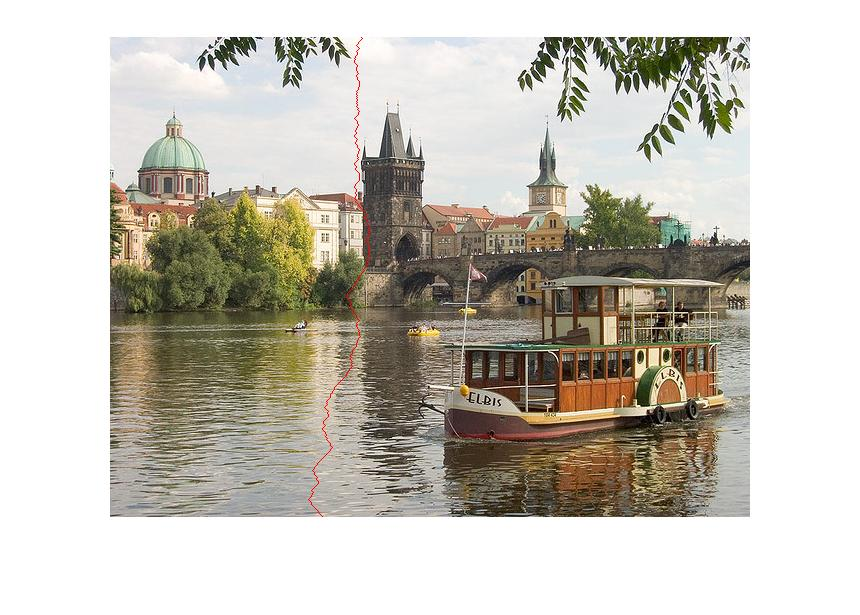
\includegraphics[width=\textwidth]
        {Problem5_vertical.jpg}}
        \caption{First horizontal seam}
      \end{figure}
\clearpage

\textbf{explain the impact:}
It goes through the cost area where there is a big giant around the seam since it is less sensitive to the difference of cost energy now. Comparing it the original function, it is less sensitive to the energy gap areas.



\clearpage
\begin{subsection}{II.6}

\begin{subsubsection}{Sample 1}
\begin{figure}[!htb]
        \center{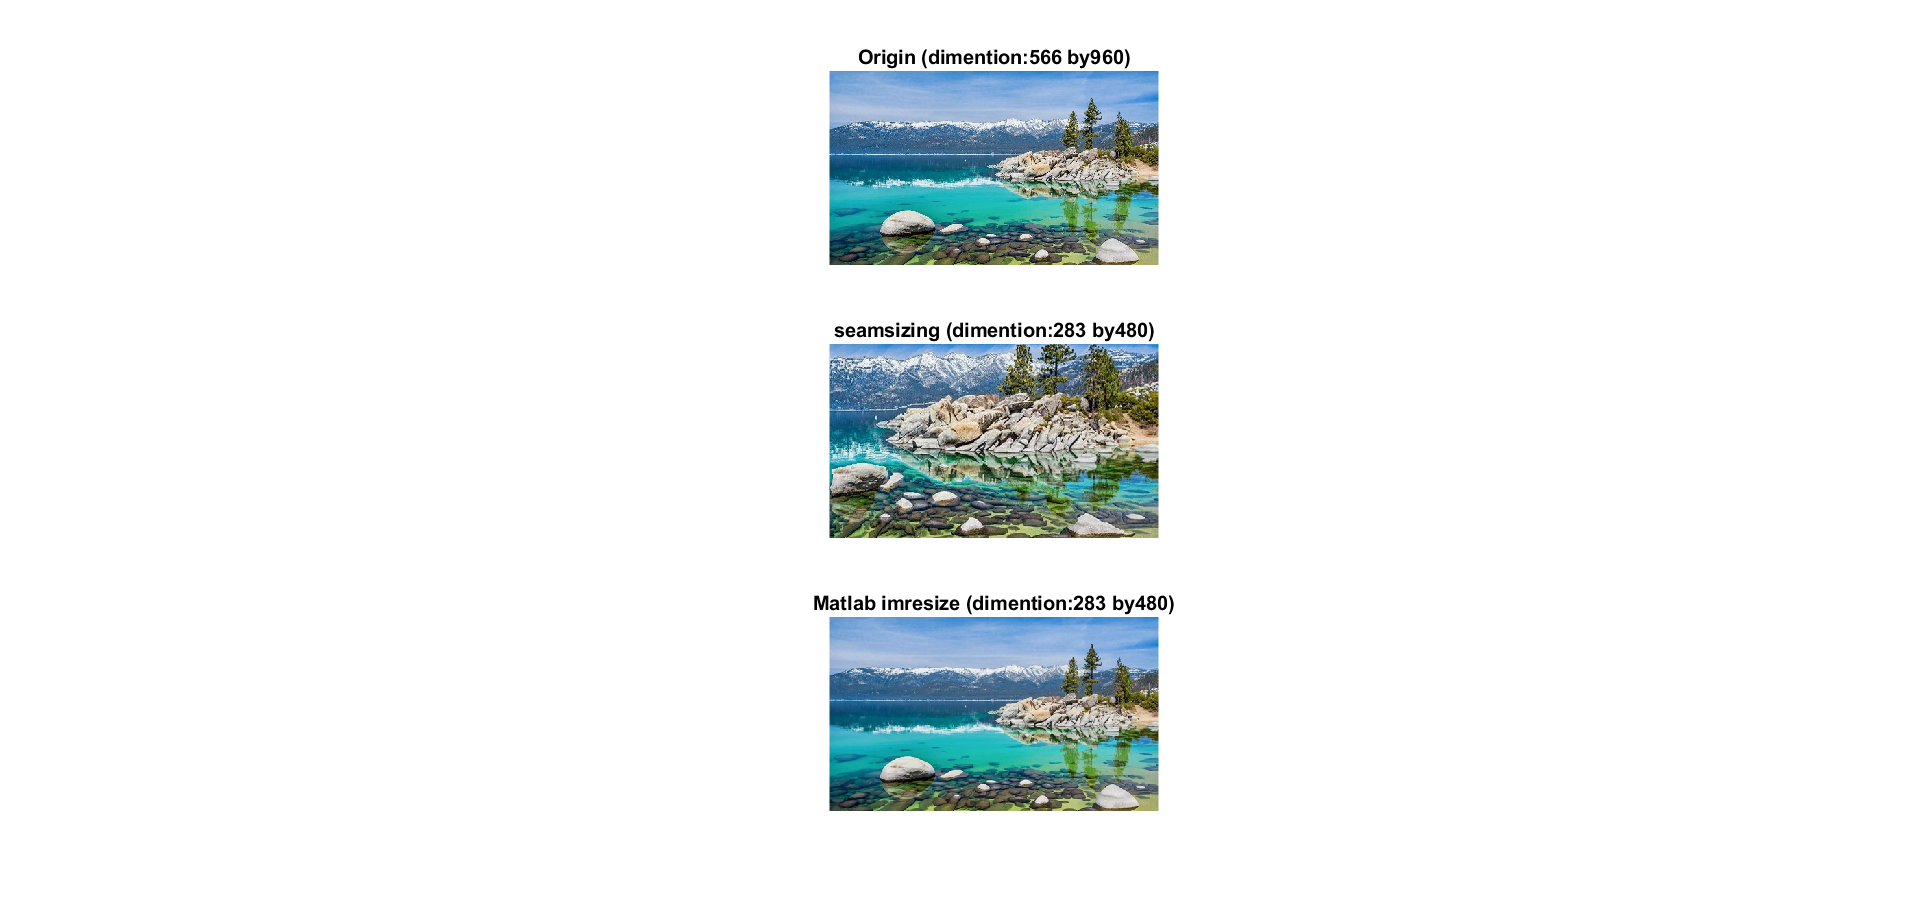
\includegraphics[width=\textwidth]
        {pro6_tahoe.png}}
        \caption{Lake Thoe (sources:  https://www.forbes.com/sites/trevornace/2018/04/05/snowiest-march-in-decades-fills-lake-tahoe-with-enough-water-for-three-years/\#1263829f7053)
}
\end{figure}

\textbf{Sequence of enlargements and removals}\\
In this sample, we removed half of colums from the image first and then remove half of the rows.

\textbf{Qualitative Explanation}\\
After resizing the image by using seam carving method, elements in the image looks more closer to each other. The image is denser to look at. Overall, the image seems normal, because is large piece area (sky, lake) in the image that are ``smooth'' i.e. pixels in that area are similar, it is easy to find the carving seam and cut out the part where it looks the same without changing the overall image too much. 
\end{subsubsection}

\clearpage
\begin{subsubsection}{Sample 2}
\begin{figure}[!htb]
        \center{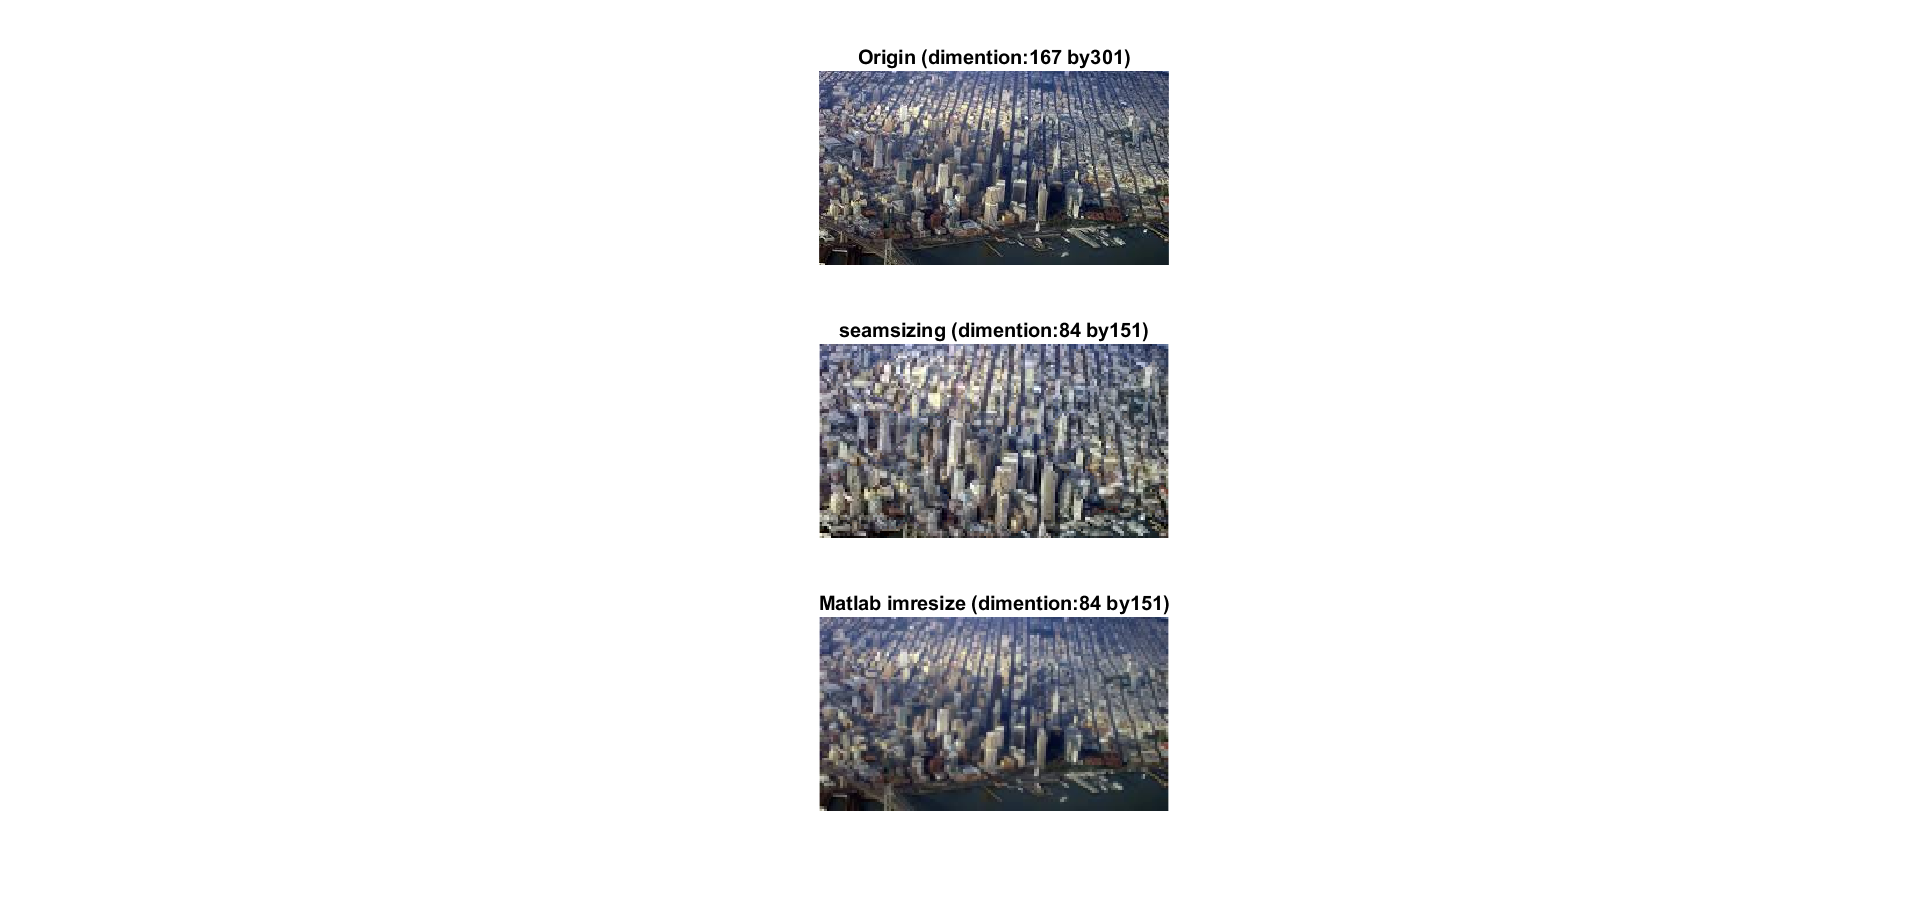
\includegraphics[width=\textwidth]
        {pro6_SF.png}}
        \caption{San Francisco (sources: https://www.modernluxury.com/san-francisco/story/san-francisco-the-second-most-dense-city-america
)
}
\end{figure}

\textbf{Sequence of enlargements and removals}\\
In this sample, we removed half of colums from the image first and then remove half of the rows.

\textbf{Qualitative Explanation}\\
In this sample, the method we used to resize the image does not reserve the part of the port from the image. But other than that, the image looks normal. The reason is because in the area of the port, the pixels look similar, so it is easier to cut that part without bringing up too much attention to the reader.

\end{subsubsection}



\clearpage
\begin{subsubsection}{Sample 3}
\begin{figure}[!htb]
        \center{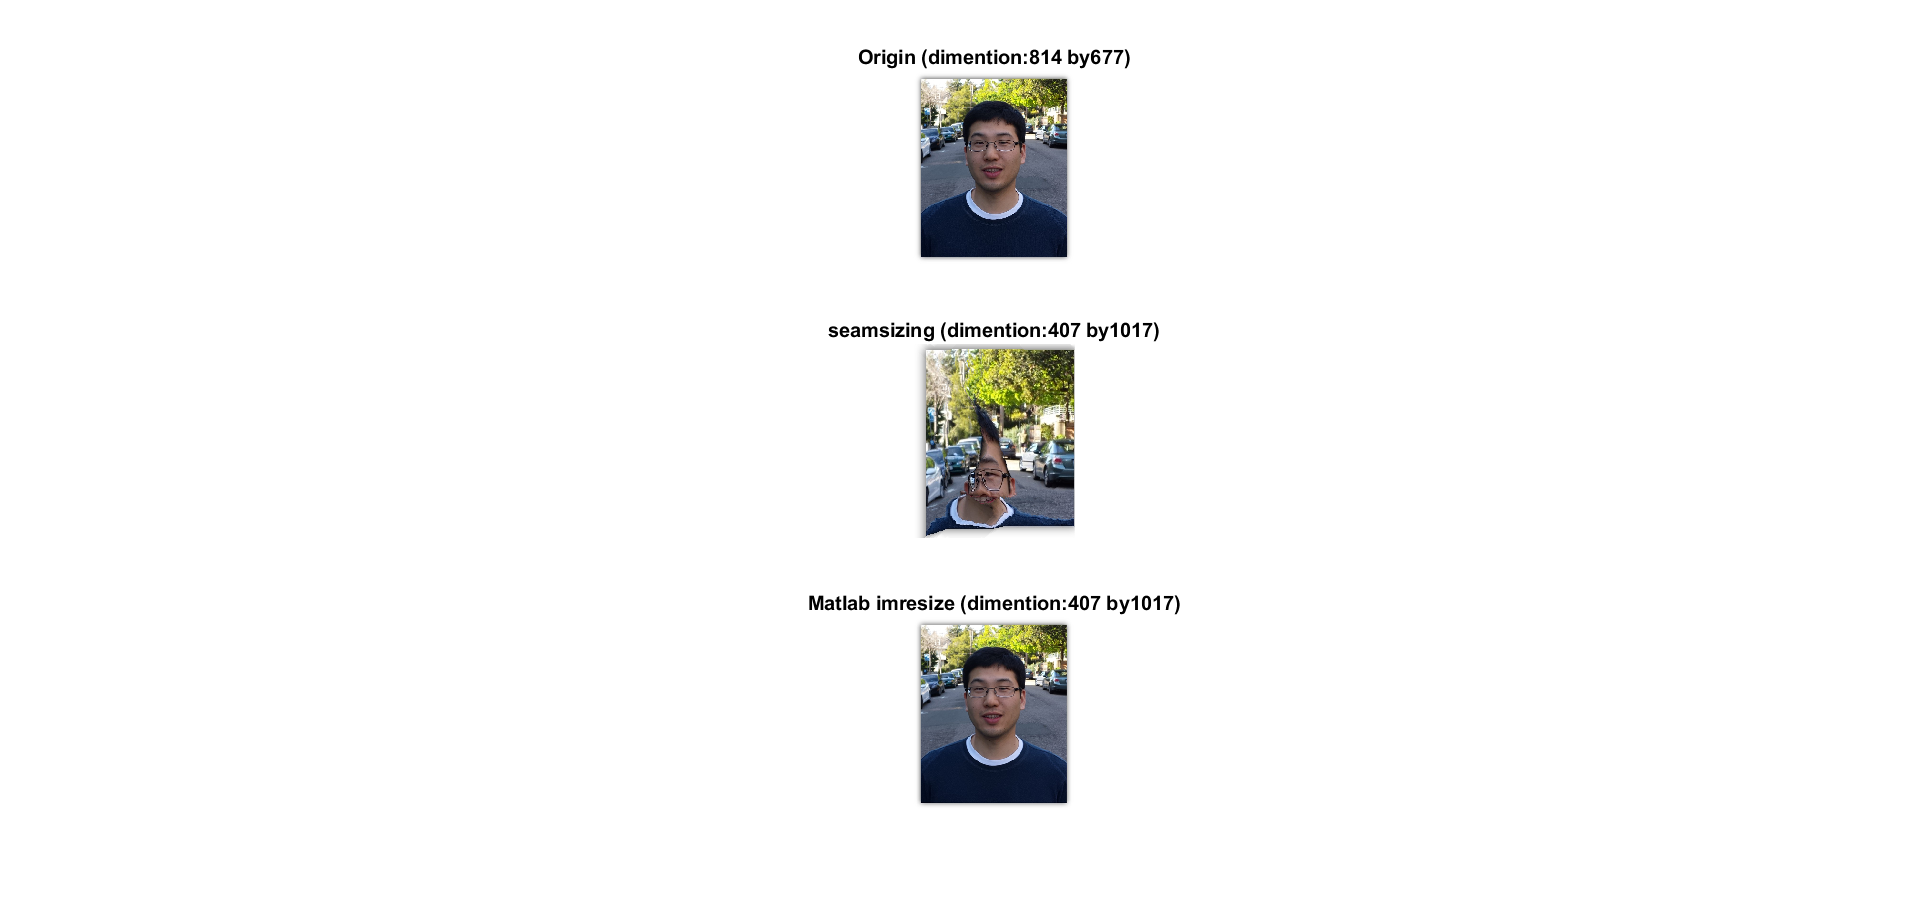
\includegraphics[width=\textwidth]
        {pro6_YJLee.png}}
        \caption{Professor Lee (https://web.cs.ucdavis.edu/~yjlee/
)
}
\end{figure}

\textbf{Sequence of enlargements and removals}\\
In this sample, we removed half of colums from the image first and then remove half of the rows.

\textbf{Qualitative Explanation}\\
In this sample, the method we used to resize the image failed. The reason would be all verticle seams and horizontal seams will go through the human part in the image, which is the essencial part of the image, thus resizing the image to 0.5 would change the image a lot.

\end{subsubsection}

\textbf{Try to predict type of images}\\
For images that have big pieces of segment that have similar pixels, the seam carving algorithm would work well. For images in which the single essential segment occupies most of the images, the algorithm does not work well. For images in which some pixels are very different at one part while similar at the other part, the similar part would be cut off. In this case, if the important part of the image appears at the ``smooth '' section of the image, the algorithm will not work well. Like in sample 2 with dense city crowd, if the port is the important part of the image, the resizing algorithm will cut out the most important part of information.

\end{subsection}

\end{subsection}


\end{section}

\clearpage
\begin{section}{Optional question}
\textbf{4. Implement the greedy solution, and compare the results to the optimal solution}

Matlab CODE:\\
greedy\_ver\_seam.m\\
\begin{lstlisting}[frame=single]  % Start your code-block
% Use Greedy solution to find the seam
% Input the result im from function energ_im
% Output the vector containing the index of selected pixel for each rows

function greedy_vertical_seam = greedy_ver_seam(im)
    [num_rows, num_col] = size(im);
    v = zeros(1,num_rows);
    [~,ind] = min(im(1,:)); 
    v(1,1) = ind;
    
    for i = 2 : num_rows
        [~,j] = min(im(1,i - 1));
        if j == 1
            [~,ind] = min([im(i,j), im(i,j+1)]);
            
            v(1,i) = ind + j - 1;
        elseif j == num_col
            [~,ind] = min([im(i,j - 1), im(i,j)]);
            v(1,i) = ind + j - 2;
        else
            [~,ind] = min([im(i,j - 1), im(i,j), im(i,j + 1)]);
            v(1,i) = ind + j - 2;
        end
        
    end
    
    
    greedy_vertical_seam = v;
end

\end{lstlisting}
greedy\_hor\_seam.m\\
\begin{lstlisting}[frame=single]  % Start your code-block
function greedy_horizontal_seam = greedy_hor_seam(im)
    im = im';
    greedy_horizontal_seam = greedy_ver_seam(im);
    
end

\end{lstlisting}

OUTPUT:\\


\begin{figure}[!htb]
        \center{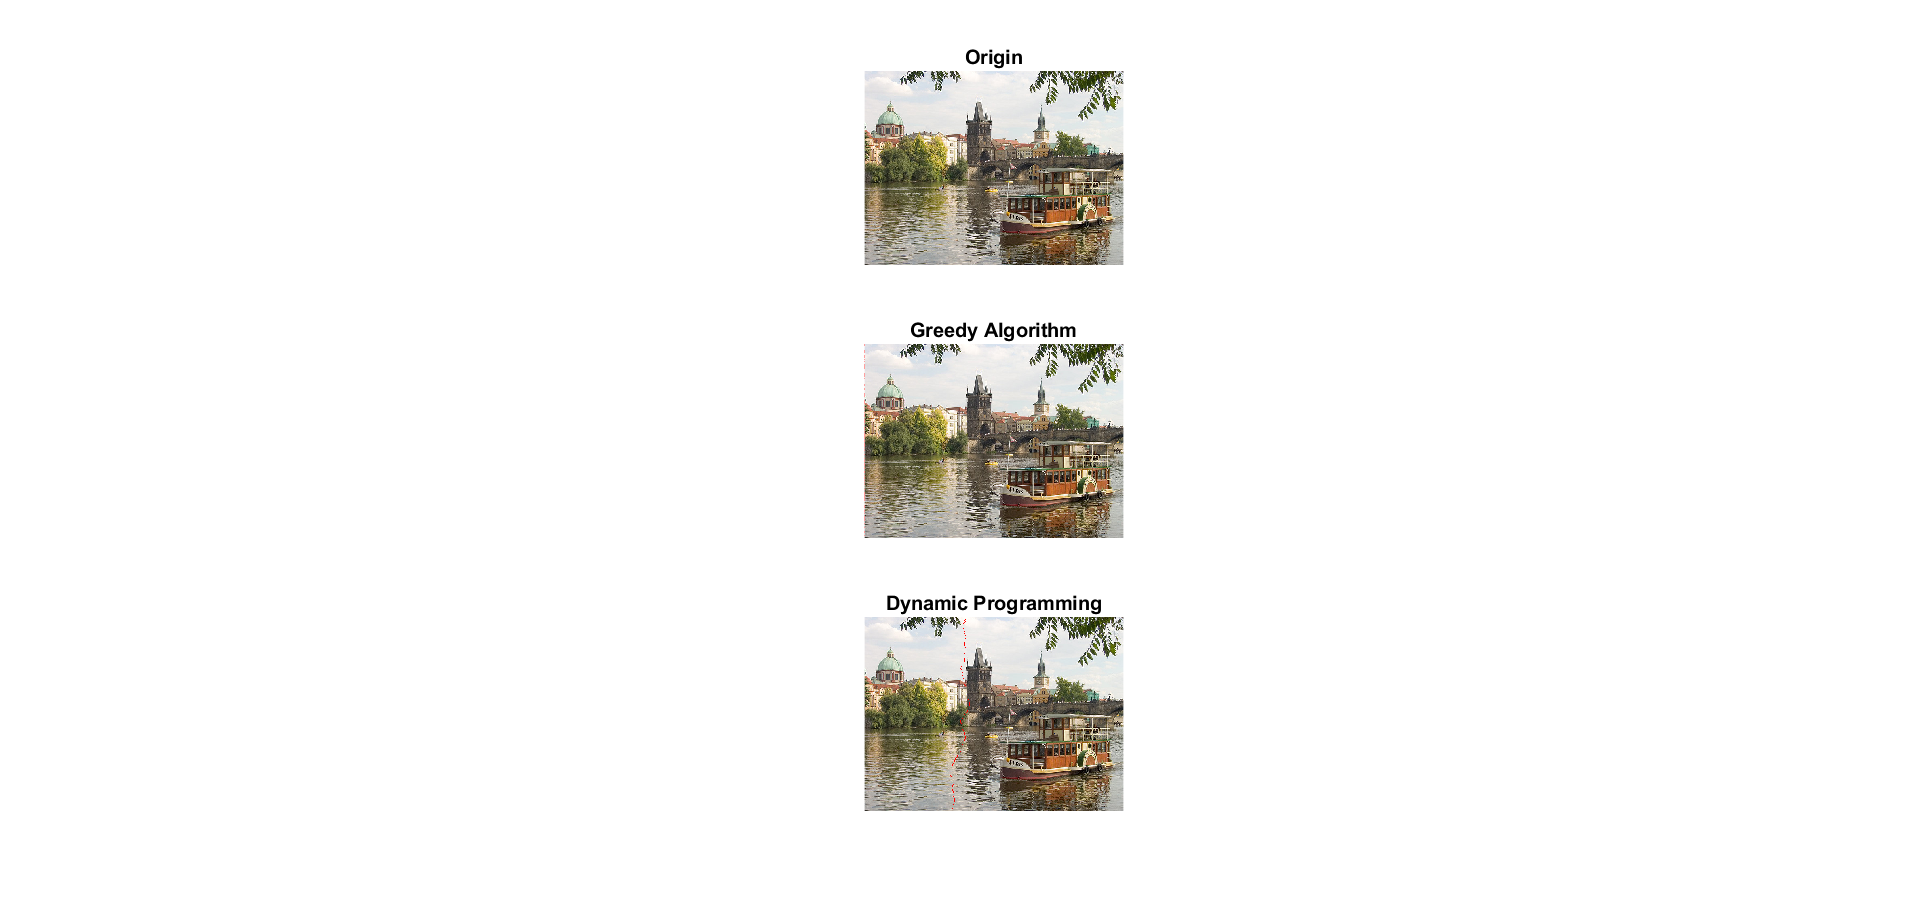
\includegraphics[width=\textwidth]
        {optional.png}}
        \caption{Comparison of greedy algorithm and dynamic programming}
      \end{figure}

As we can see from the comparison above, by using dynamic algorithm we get a vertical seam close to the middle of the image, while the greedy algorithm gives us a vertical seam close to the left most edge of the image. Greedy algorithm fails here because the minimum value in the first row of the image does not necessary need to be in the globla optimum carving seam.

\end{section}

\end{document}